\documentclass[12pt,letterpaper]{article}

\newenvironment{proof}{\noindent{\bf Proof:}}{\qed\bigskip}

\newtheorem{theorem}{Theorem}
\newtheorem{corollary}{Corollary}
\newtheorem{lemma}{Lemma} 
\newtheorem{claim}{Claim}
\newtheorem{fact}{Fact}
\newtheorem{definition}{Definition}
\newtheorem{assumption}{Assumption}
\newtheorem{observation}{Observation}
\newtheorem{example}{Example}
\newcommand{\qed}{\rule{7pt}{7pt}}

\newcommand{\assignment}[4]{
\thispagestyle{plain} 
\newpage
\setcounter{page}{1}
\noindent
\begin{center}
\framebox{ \vbox{ \hbox to 6.28in
{\bf CS446: Machine Learning \hfill #1}
\vspace{4mm}
\hbox to 6.28in
{\hspace{2.5in}\large\mbox{Problem Set #2}}
\vspace{4mm}
\hbox to 6.28in
{{\it Handed Out: #3 \hfill Due: #4}}
}}
\end{center}
}

\newcommand{\solution}[4]{
\thispagestyle{plain} 
\newpage
\setcounter{page}{1}
\noindent
\begin{center}
\framebox{ \vbox{ \hbox to 6.28in
{\bf CS446: Machine Learning \hfill #4}
\vspace{4mm}
\hbox to 6.28in
{\hspace{2.5in}\large\mbox{Problem Set #3}}
\vspace{4mm}
\hbox to 6.28in
{#1 \hfill {\it Handed In: #2}}
}}
\end{center}
\markright{#1}
}

\newenvironment{algorithm}
{\begin{center}
\begin{tabular}{|l|}
\hline
\begin{minipage}{1in}
\begin{tabbing}
\quad\=\qquad\=\qquad\=\qquad\=\qquad\=\qquad\=\qquad\=\kill}
{\end{tabbing}
\end{minipage} \\
\hline
\end{tabular}
\end{center}}

\def\Comment#1{\textsf{\textsl{$\langle\!\langle$#1\/$\rangle\!\rangle$}}}


\usepackage{graphicx,amsmath,amssymb,url,epstopdf}
\sloppy
\oddsidemargin 0in
\evensidemargin 0in
\textwidth 6.5in
\topmargin -0.5in
\textheight 9.0in

\newcommand{\bb}[1]{\bf #1}
\newcommand{\ignore}[1]{}
\newcommand{\pp}{\noindent}
\newcommand{\ov}{\overline}
\renewcommand{\labelitemii}{\tiny$\circ$}

\begin{document}

\assignment{Fall 2014}{5}{October $28^{th}$, $2014$}{November $06^{th}$, $2014$}
\begin{footnotesize}
\begin{itemize}

\item Feel free to talk to other members of the class in doing the homework.  I am
more concerned that you learn how to solve the problem than that you
demonstrate that you solved it entirely on your own.  You should, however,
write down your solution yourself.  Please try to keep the solution brief and
clear.
\item Please use Piazza first if you have questions about the homework.
  Also feel free to send us e-mails and come to office hours.

\item Please, no handwritten solutions.

\item The homework is due at 11:59 PM on the due date. Please submit your solution manuscript as a single pdf file via Compass
(\texttt{http://compass2g.illinois.edu}).

\item No code is needed for any of these problems. You can do the
calculations however you please. You need to turn in only the report.

\end{itemize}
\end{footnotesize}

\begin{enumerate}

\item {\bf [SVM - 50 points]}

\pp
We have a set of six labeled examples $D$ in the two-dimensional space, $D = \{(\mathbf{x}^{(1)}, y^{(1)}),...,(\mathbf{x}^{(6)}, y^{(6)})\}$, $\mathbf{x}^{(i)} \in \mathbb{R}^{2}$ and $y^{(i)} \in \{1, -1\}, i=1,2,...,6$ listed as follows:
  \begin{center}
    \begin{tabular}{|c|c|c|c|}
      \hline
      {\em i}  & $\mathbf{x}_1^{(i)}$  & $\mathbf{x}_2^{(i)}$ & $y^{(i)}$ \\
      \hline
      {\em 1}  & $-1.2$  & $1.6$ & $1$ \\
      \hline
      {\em 2}  & $-1.6$  & $2$ & $1$ \\
      \hline
      {\em 3}  & $4$  & $1$ & $-1$ \\
      \hline
      {\em 4}  & $-3$  & $0$ & $1$ \\
      \hline
      {\em 5}  & $3$  & $-0.8$ & $-1$ \\
      \hline
      {\em 6}  & $2$  & $0$ & $-1$ \\
      \hline
    \end{tabular}
  \end{center}
  \begin{figure}[h!]
        \begin{center}
          \includegraphics[width=0.7\textwidth]{3.eps}
          \caption{Examples}
          \label{fig:1-500}
        \end{center}
      \end{figure}
\begin{enumerate}
% (a)
\item[(a)][$20$ points]
We want to find a linear classifier where examples $\mathbf{x}$ are positive if and only if $\mathbf{w}\cdot \mathbf{x} + \theta \geq 0$.

\begin{enumerate}
% 1.
\item[1.][$3$ points] Find an easy solution $(\mathbf{w}, \theta)$ that can separate the positive and negative examples given.

\vspace{.13in}
Define $\mathbf{w}=$ $\underline{\qquad\qquad\qquad\qquad}$

\vspace{.13in}
Define $\theta =$ $\underline{\qquad\qquad\qquad\qquad}$
\vspace{.13in}
% 2.
\item[2.][$10$ points] Recall the Hard SVM formulation:
%\begin{equation}
\begin{gather}
\textbf{min}_{\mathbf{w}}\frac{1}{2}||\mathbf{w}||^2 \\
\text{s.t  } y^{(i)}(\mathbf{w}\cdot\mathbf{x}^{(i)}+\theta)\geq 1, \forall (\mathbf{x}^{(i)},y^{(i)})\in D
\end{gather}
%\end{equation}

What would the solution be if you solve this optimization problem? (Note: you don't actually need to solve the optimization problem; we expect that you can use simple analytic geometry to derive the same solution SVM would derive).

\vspace{.13in}
Define $\mathbf{w}=$ $\underline{\qquad\qquad\qquad\qquad}$

\vspace{.13in}
Define $\theta =$ $\underline{\qquad\qquad\qquad\qquad}$
\vspace{.13in}

\item[3.][$7$ points] Given your understanding of SVM optimization, how did you derive the SVM solution for the points in Figure 1?

\vspace{.60in}

\end{enumerate}

% (b)
\item[(b)][$17$ points]
Recall the dual representation of SVM. There exists coefficients $\alpha_{i} > 0$ such that:
\begin{eqnarray}
\mathbf{w}^{*} = \sum_{i\in I}{\alpha_{i}y^{(i)}\mathbf{x}^{(i)}}
\end{eqnarray}
where $I$ is the set of indices of the support vectors.
\begin{enumerate}

% 1.
\item[1.][$5$ points] Identify support vectors from the six examples given.

\vspace{.2in}
Define $I =$ $\underline{\qquad\qquad\qquad\qquad}$
\vspace{.2in}


% 2.
\item[2.][$6$ points] For the support vectors you have identified, find $\alpha_i$ such that the dual representation of $\mathbf{w}^{*}$ is equal to the primal one you found in (a)-2.

 \vspace{.2in}
Define $\mathbf{\alpha} = \{\alpha_1, \alpha_2, ..., \alpha_{|I|}\} = $ $\underline{\qquad\qquad\qquad\qquad}$
\vspace{.2in}

% 3.
%\item[3.][$3$ points] Recall the objective function for primal representation of SVM.
%\begin{eqnarray}
%Primal: \textbf{min }   \frac{1}{2}||\mathbf{w}||^{2} + C\sum_{j=1}^{m}{max(0, 1-y^{(j)}(\mathbf{w}\cdot\mathbf{x}^{(j)}+ \theta))}
%\end{eqnarray}

 \vspace{.2in}

\vspace{.2in}

\item[3.][$6$ points] Compute the value of the hard SVM objective function for the optimal solution you found.


 \vspace{.2in}
\emph{Objective function value} =  $\underline{\qquad\qquad\qquad\qquad}$
\vspace{.2in}
\end{enumerate}

% (c)
\item[(c)][$13$ points] Recall the objective function for soft representation of SVM.
\begin{gather}
\textbf{min }   \frac{1}{2}||\mathbf{w}||^{2} + C\sum_{j=1}^{m}{\xi_{i}} \\
\text{s.t  } y^{(i)}(\mathbf{w}\cdot\mathbf{x}^{(i)}+\theta)\geq 1 - \xi_{i}, \xi_i\geq0, \forall (\mathbf{x}^{(i)},y^{(i)})\in D
\end{gather}

where $m$ is the number of examples. Here $C$ is an important parameter. What is the meaning of it? For which value of $C$, the solution to this optimization problem gives the hyperplane that achieves the largest margin (i.e., the hyperplane you have found in (a)-2? Comment on the impact on the margin and support vectors when we use $C = \infty$, $C = 1$, and $C = 0$.
\vspace{.7in}

\end{enumerate}

\item {\bf [Kernels - 15 points]}
  \begin{enumerate}
  \item {\bf [5 points]} Write down the dual representation of the
    Perceptron algorithm.

  \item {\bf [5 points]} If $K_1(\vec{\bb{x}},\vec{\bb{z}})$ and
    $K_2(\vec{\bb{x}},\vec{\bb{z}})$ are both valid kernel functions, with
    positive $\alpha$ and $\beta$, prove that
    \begin{equation*}
      K(\vec{\bb{x}},\vec{\bb{z}}) = \alpha K_1(\vec{\bb{x}},\vec{\bb{z}}) + \beta K_2(\vec{\bb{x}},\vec{\bb{z}})
    \end{equation*}
    is also a kernel function.

  \item {\bf [5 points]} Given two examples $\vec{\bb{x}} \in \mathbb{R}^2$ and
    $\vec{\bb{z}} \in \mathbb{R}^2$, let
    \begin{equation*}
      K(\vec{\bb{x}},\vec{\bb{z}}) = (\vec{\bb{x}}^T\vec{\bb{z}})^3 + 400(\vec{\bb{x}}^T\vec{\bb{z}})^2 + 100 \vec{\bb{x}}^T\vec{\bb{z}}.
    \end{equation*}
    Prove that this is a valid kernel function.

  \end{enumerate}

\item {\bf [Boosting - 30 points]}
  Consider the following examples $(x,y) \in \mathbb{R}^2$ ({\em i} is the example index):
  \begin{center}
    \begin{tabular}{|c|c|c|c|}
      \hline
      {\em i}  & $x$  & $y$ & Label \\
      \hline
      {\em 1}  & 1  & 10 & $-$ \\
      \hline
      {\em 2}  & 4  & 4 & $-$ \\
      \hline
      {\em 3}  & 8  & 7 & $+$ \\
      \hline
      {\em 4}  & 5  & 6 & $-$ \\
      \hline
      {\em 5}  & 3  & 16 & $-$ \\
      \hline
      {\em 6}  & 7  & 7 & $+$ \\
      \hline
      {\em 7}  & 10 & 14 & $+$ \\
      \hline
      {\em 8}  & 4  & 2 & $-$ \\
      \hline
      {\em 9}  & 4  & 10 & $+$ \\
      \hline
      {\em 10} & 8  & 8 & $-$ \\
      \hline
    \end{tabular}
  \end{center}
    % {\bf Add indices to the rows of both tables?}

    \begin{table}[!t]
      {\centering
        \begin{tabular}{|c|c||c|c|c|c||c|c|c|c|}

          \hline
          & & \multicolumn{4}{c||}{Hypothesis 1}
	  & \multicolumn{4}{c|}{Hypothesis 2} \\
          \cline{3-10}
          {\em i} & Label & $D_0$ & $x_1 \equiv $ & $x_2 \equiv $ & $h_1\equiv$ & $D_1$ &  $x_1 \equiv $ & $x_2 \equiv $ & $h_2 \equiv $ \\
          & & & [$x >$\rule[-2pt]{3mm}{0.2pt}$\;$] & [$y >$\rule[-2pt]{3mm}{0.2pt}$\;$] & [$\;$\rule[-2pt]{1cm}{0.2pt}$\;$] & & [$x >$\rule[-2pt]{3mm}{0.2pt}$\;$] & [$y >$\rule[-2pt]{3mm}{0.2pt}$\;$] & [$\;$\rule[-2pt]{1cm}{0.2pt}$\;$] \\

          \tiny{(1)} & \tiny{(2)} & \tiny{(3)} & \tiny{(4)} &  \tiny{(5)} & \tiny{(6)} & \tiny{(7)} & \tiny{(8)} & \tiny{(9)} & \tiny{(10)}\\
          \hline \hline
          {\em 1} & $-$ & & & & & & & &  \\
          \hline
          {\em 2} & $-$ & & & & & & & &  \\
          \hline
          {\em 3} & $+$ & & & & & & & & \\
          \hline
          {\em 4} & $-$ & & & & & & & & \\
          \hline
          {\em 5} & $-$ & & & & & & & & \\
          \hline
          {\em 6} & $+$ & & & & & & & & \\
          \hline
          {\em 7} & $+$ & & & & & & & & \\
          \hline
          {\em 8} & $-$ & & & & & & & & \\
          \hline
          {\em 9} & $+$ & & & & & & & & \\
          \hline
          {\em 10} & $-$ & & & & & & & & \\
          \hline
        \end{tabular}
        \caption{Table for Boosting results} \label{table:ltu}}
    \end{table}


  In this problem, you will use Boosting to learn a hidden Boolean function from this set of examples.
We will use two rounds of AdaBoost to learn a hypothesis for this
    data set. In each round, AdaBoost chooses a weak learner that minimizes the error $\epsilon$. As weak learners, use hypotheses of the form (a)~$x_1 \equiv [x
    > \theta_x]$ or (b)~$x_2 \equiv [y > \theta_y]$, for some integers $\theta_x, \theta_y$ (either one of the two forms, not a disjunction of the two). There should be no need to try many values of $\theta_x, \theta_y$;
    appropriate values should be clear from the data.


  \begin{enumerate}
  \item {\bf [6 points]}  Start the first round with a uniform distribution $D_0$.  Place the value for
    $D_0$ for each example in the third column of Table~\ref{table:ltu}.
Write the new representation of the data in terms of the {\em rules of thumb}, $x_1$ and $x_2$, in the fourth and fifth columns of Table~\ref{table:ltu}.

  \item {\bf [6 points]}
    Find the hypothesis given by the weak learner that minimizes the error
    $\epsilon$ for that distribution.  Place this hypothesis as the heading to the
    sixth column of Table~\ref{table:ltu}, and give its prediction for each example in that column.

   \item {\bf [6 points]} Now compute $D_1$ for each example, find the new best weak learners $x_1$ and $x_2$, and select hypothesis that
    minimizes error on this distribution, placing these values and
    predictions in the seventh to tenth columns of Table~\ref{table:ltu}.

  \item {\bf [6 points]} Write down the final hypothesis produced by AdaBoost.

  \item {\bf [6 points]} Prove or disprove: AdaBoost determines
    the distribution at time $t+1$ in such a way that the error of the $t-$th hypothesis
    is exactly half.

%  \item Use the Perceptron learning algorithm to train a hypothesis for this Boolean
%   data set, using as features the weak learners chosen by the boosting algorithm in (a).
%
%    Train the Perceptron one cycle through the data, setting initial weights as $0$,
%    the threshold as $3$, and the learning rate as $1$. Fill in the ninth column
%   (labeled \texttt{weight vector}) of Table~\ref{table:ltu}.
%
%
%  \item Did the two algorithms converge to the same hypothesis?  Explain (or give an example).

\end{enumerate}

\textbf{What to submit:} Fill out Table~\ref{table:ltu} as explained, show computation of $\alpha$ and $D_1(i)$, give the final hypothesis, $H_{\textit{final}}$, and state your answer to part (e).


%\item {\bf [Multi-class classification - 20 points]}
%
%Consider a multi-class classification problem with $k$ class
%labels $\{1, 2, \ldots k\}$. Assume that we are given $m$
%examples, labeled with one of the $k$ class labels. Assume, for
%simplicity, that we have $m/k$ examples of each type.
%
%Assume that you have a learning algorithm $L$ that can be used
%to learn Boolean functions. (E.g., think about $L$ as the
%Perceptron algorithm). We would like to explore several ways to
%develop learning algorithms for the multi-class classification
%problem.
%
%There are two schemes to use the algorithm $L$ on the given data set, and produce a multi-class classification:
%\begin{itemize}
%\item {\bf One vs.~All:} For every label $i \in [1,k]$, a classifier is learned over the following data set: the examples labeled with the label $i$ are considered ``positive'', and examples labeled with any other class $j \in [1,k], j \neq i$ are considered ``negative''.
%\item {\bf All vs.~All:} For every pair of labels $\langle i, j \rangle$, a classifier is learned over the following data set: the examples labeled with one class $i \in [1,k]$ are considered ``positive'', and those labeled with the other class $j \in [1,k], j \neq i$ are considered ``negative''.
%\end{itemize}
%%
%\vspace{-3mm}
%\begin{enumerate}
%\item {\bf [10 points]} For each of these two schemes, answer the following:
%\begin{enumerate}
%\item How many classifiers do you learn?
%\item How many examples do you use to learn each classifier within the scheme?
%\item How will you decide the final class label (from \{1, 2, \ldots, k\}) for each example?
%\item What is the computational complexity of the training process?
%\end{enumerate}
%\item {\bf [5 points]} Based on your analysis above of two schemes individually, which scheme would you prefer? Justify.
%\item {\bf [5 points]} In Problem Set $4$, we asked you to write a \textsc{KernelPerceptron} for a two-class classification. We could also use the algorithm to learn a multi-class classification. Does using a \textsc{KernelPerceptron} change your analysis above? Specifically, what is the computational complexity of using a \textsc{KernelPerceptron} and which scheme would you prefer when using a \textsc{KernelPerceptron}?
%\end{enumerate}

\item {\bf [Probability - 5 points]}
\begin{enumerate}

\item {\bf [5 points]} There are two towns A and B, where all families follow the following scheme for family planning:
\begin{itemize}
\item Town A: Each family has just one child -- either a boy or a girl.
\item Town B: Each family has as many children as it wants, until a boy is born, and then it does not have any more children.
\end{itemize}
Assume that the boy to girl ratio is 1:1 for both towns A and B (number of boys equals number of girls), and the probability of having a boy child is 0.5, the same as that of having a girl child. Answer the following questions:
\begin{enumerate}
\item What is the expected number of children in a family in towns A and B?
\item What is the boy to girl ratio at the end of one generation in towns A and B?
\end{enumerate}
\end{enumerate}

\end{enumerate}

\end{document}
